\documentclass[journal, a4paper]{IEEEtran}

% some very useful LaTeX packages include:
\usepackage[brazil]{babel}
\usepackage[utf8x]{inputenc}
\usepackage{amsmath}
\usepackage{float}
\usepackage{mathtools}
\usepackage{natbib}
%\usepackage{multicol, blindtext}

%\usepackage{cite}      % Written by Donald Arseneau
                        % V1.6 and later of IEEEtran pre-defines the format
                        % of the cite.sty package \cite{} output to follow
                        % that of IEEE. Loading the cite package will
                        % result in citation numbers being automatically
                        % sorted and properly "ranged". i.e.,
                        % [1], [9], [2], [7], [5], [6]
                        % (without using cite.sty)
                        % will become:
                        % [1], [2], [5]--[7], [9] (using cite.sty)
                        % cite.sty's \cite will automatically add leading
                        % space, if needed. Use cite.sty's noadjust option
                        % (cite.sty V3.8 and later) if you want to turn this
                        % off. cite.sty is already installed on most LaTeX
                        % systems. The latest version can be obtained at:
                        % http://www.ctan.org/tex-archive/macros/latex/contrib/supported/cite/

\usepackage{graphicx}   % Written by David Carlisle and Sebastian Rahtz
                        % Required if you want graphics, photos, etc.
                        % graphicx.sty is already installed on most LaTeX
                        % systems. The latest version and documentation can
                        % be obtained at:
                        % http://www.ctan.org/tex-archive/macros/latex/required/graphics/
                        % Another good source of documentation is "Using
                        % Imported Graphics in LaTeX2e" by Keith Reckdahl
                        % which can be found as esplatex.ps and epslatex.pdf
                        % at: http://www.ctan.org/tex-archive/info/

\usepackage{psfrag}    % Written by Craig Barratt, Michael C. Grant,
                        % and David Carlisle
                        % This package allows you to substitute LaTeX
                        % commands for text in imported EPS graphic files.
                        % In this way, LaTeX symbols can be placed into
                        % graphics that have been generated by other
                        % applications. You must use latex->dvips->ps2pdf
                        % workflow (not direct pdf output from pdflatex) if
                        % you wish to use this capability because it works
                        % via some PostScript tricks. Alternatively, the
                        % graphics could be processed as separate files via
                        % psfrag and dvips, then converted to PDF for
                        % inclusion in the main file which uses pdflatex.
                        % Docs are in "The PSfrag System" by Michael C. Grant
                        % and David Carlisle. There is also some information
                        % about using psfrag in "Using Imported Graphics in
                        % LaTeX2e" by Keith Reckdahl which documents the
                        % graphicx package (see above). The psfrag package
                        % and documentation can be obtained at:
                        % http://www.ctan.org/tex-archive/macros/latex/contrib/supported/psfrag/

\usepackage{subfig} % Written by Steven Douglas Cochran
                        % This package makes it easy to put subfigures
                        % in your figures. i.e., "figure 1a and 1b"
                        % Docs are in "Using Imported Graphics in LaTeX2e"
                        % by Keith Reckdahl which also documents the graphicx
                        % package (see above). subfigure.sty is already
                        % installed on most LaTeX systems. The latest version
                        % and documentation can be obtained at:
                        % http://www.ctan.org/tex-archive/macros/latex/contrib/supported/subfigure/

\usepackage{url}        % Written by Donald Arseneau
                        % Provides better support for handling and breaking
                        % URLs. url.sty is already installed on most LaTeX
                        % systems. The latest version can be obtained at:
                        % http://www.ctan.org/tex-archive/macros/latex/contrib/other/misc/
                        % Read the url.sty source comments for usage information.

\usepackage{stfloats}  % Written by Sigitas Tolusis
                        % Gives LaTeX2e the ability to do double column
                        % floats at the bottom of the page as well as the top.
                        % (e.g., "\begin{figure*}[!b]" is not normally
                        % possible in LaTeX2e). This is an invasive package
                        % which rewrites many portions of the LaTeX2e output
                        % routines. It may not work with other packages that
                        % modify the LaTeX2e output routine and/or with other
                        % versions of LaTeX. The latest version and
                        % documentation can be obtained at:
                        % http://www.ctan.org/tex-archive/macros/latex/contrib/supported/sttools/
                        % Documentation is contained in the stfloats.sty
                        % comments as well as in the presfull.pdf file.
                        % Do not use the stfloats baselinefloat ability as
                        % IEEE does not allow \baselineskip to stretch.
                        % Authors submitting work to the IEEE should note
                        % that IEEE rarely uses double column equations and
                        % that authors should try to avoid such use.
                        % Do not be tempted to use the cuted.sty or
                        % midfloat.sty package (by the same author) as IEEE
                        % does not format its papers in such ways.

\usepackage{amsmath}    % From the American Mathematical Society
                        % A popular package that provides many helpful commands
                        % for dealing with mathematics. Note that the AMSmath
                        % package sets \interdisplaylinepenalty to 10000 thus
                        % preventing page breaks from occurring within multiline
                        % equations. Use:
\interdisplaylinepenalty=2500
                        % after loading amsmath to restore such page breaks
                        % as IEEEtran.cls normally does. amsmath.sty is already
                        % installed on most LaTeX systems. The latest version
                        % and documentation can be obtained at:
                        % http://www.ctan.org/tex-archive/macros/latex/required/amslatex/math/



% Other popular packages for formatting tables and equations include:

%\usepackage{array}
% Frank Mittelbach's and David Carlisle's array.sty which improves the
% LaTeX2e array and tabular environments to provide better appearances and
% additional user controls. array.sty is already installed on most systems.
% The latest version and documentation can be obtained at:
% http://www.ctan.org/tex-archive/macros/latex/required/tools/

% V1.6 of IEEEtran contains the IEEEeqnarray family of commands that can
% be used to generate multiline equations as well as matrices, tables, etc.

% Also of notable interest:
% Scott Pakin's eqparbox package for creating (automatically sized) equal
% width boxes. Available:
% http://www.ctan.org/tex-archive/macros/latex/contrib/supported/eqparbox/

% *** Do not adjust lengths that control margins, column widths, etc. ***
% *** Do not use packages that alter fonts (such as pslatex).         ***
% There should be no need to do such things with IEEEtran.cls V1.6 and later.


% Your document starts here!
\begin{document}

% Define document title and author
	\title{Relatório de Previsão de Séries Temporais}
	\author{Victor Carreira
	\thanks{Professora: Marley. Eng. Elétrica. PUC-RIO}}
	\markboth{Trabalho 02}{}
	\maketitle

% Write abstract here
\begin{abstract}
	Este relatório apresenta o resultado da previsão realizada por uma rede neural artificial \textit{Multi Layer Perceptron} do tipo \textit{Back Propagation} em um banco de dados da concessionária de energia elétrica, Light, com o intuito de se fazer a previsão mensal da sensação térmica das diversas regiões ou unidades geográficas que fazem parte da sua área de abrangência. A análise de $9$ experimentos realizados indicam que o melhor resultado da rede apresentou erros de MAPE de $3.3669$ para o conjunto de validação e $4.3468$ para o conjunto de treinamento. E valores de RMSE de $1.5717$ para o conjunto de validação e $2.3305$ para o conjunto de treinamento.
\end{abstract}


\section{Introdução}
    As Redes Neurais Artificiais (RNA) são inspiradas em modelos sensoriais do processamento de tarefas realizadas pelo cérebro \citep{Hagan1996}. Uma RNA, portanto pode ser criada através da aplicação de algoritmos matemáticos que imitem a tarefa realizada por um neurônio \citep{Nedjah2016}. Uma rede neural artificial possui semelhanças com a rede biológica presente no sistema nervoso central, neste o cômputo de informações realizado do cérebro é feito através de uma vasta quantidade de neurônios interconectados \citep{Feldman1988,Poulton2002}. A comunicação entre essas células é realizada através de impulsos elétricos. Estes são transmitidos e recebidos por meio de sinapses nervosas entre axônios e dendritos. As sinapses são estruturas elementares e uma unidade funcional localizada entre dois neurônios \citep{Krogh2008}.

	\citet{McCulloch1943} redigem o trabalho pioneiro onde foi modelado um neurônio cuja resposta dependia do \textit{input}\footnote{Valor de entrada} que provinha de outros neurônios e do peso utilizado.  Já \citet{Rosenblatt1962} cria a teoria de convergência do \textit{Perceptron} onde ele prova que modelos de neurônios possuem propriedades similares ao cérebro humano \citep{Kanal2001}. Neste sentido as rede neuronais artificiais podem realizar performasses sofisticadas no reconhecimento de padrões, mesmo se alguns neurônios forem destruídos \citep{Levy1997}. \citet{Minsky1969} demonstraram que um único  \textit{Perceptron} somente resolve uma classe muito limitada de problemas que podem ser linearizados.
	
	A retropropagação é uma técnica específica para implementar a decida do gradiente no espaço de pesos para um rede de múltiplas camadas alimentada. A ideia básica é calcular as derivadas parciais de uma função aproximativa $F(\textbf{w},\textbf{x})$ realizada pela rede em relação a todos os elementos do vetor de ajuste de pesos $\textbf{w}$ para um dado valor de entrada $\textbf{x}$ \citep{Haykin1999}.
	
	Neste relatório são apresentados os resultados do Trabalho 02 MLP de Previsão de Séries Temporais da disciplina ELE 2394, Redes Neurais I, da Engenharia elétrica.
	

% Main Part
\section{Objetivo e Metodologia}


As concessionárias de energia elétrica compram energia baseada na demanda futura. É notório que o clima (temperatura, precipitação, umidade relativa do ar, vento, etc) afeta o consumo de energia elétrica, principalmente o consumo de energia elétrica das classes residencial e comercial. A Light é uma concessionária caracterizada pelo consumo dessas duas classes. Esta característica fica evidente no caso de algumas regiões da Light, onde o percentual de clientes residenciais e comerciais é maior do que $90\%$.

A Light está situada no estado do Rio de Janeiro, e por isso apresenta grandes diversidades
climáticas dentro da sua área de concessão devido à proximidade do mar e à presença de montanhas. Portanto, estudar os efeitos do clima em relação à energia faturada e à carga é
fundamental para aumentar a eficácia na previsão do volume de consumo e, consequentemente, o
volume de compra de energia. Assim, uma das metas a serem atingidas pelas concessionárias é reduzir os erros nas estimativas da carga, reduzindo os prejuízos na compra de energia. Dessa forma, a empresa poderá reduzir o risco no fluxo de caixa permitindo futuros investimentos na expansão e qualidade dos serviços prestados a seus clientes.

Portanto, o objetivo deste trabalho é desenvolver um modelo para a previsão mensal da sensação
térmica das diversas regiões ou unidades geográficas que fazem parte da área de concessão da
Light.

A partir do modelo de previsão da sensação térmica se poderá desenvolver um modelo original de
previsão de carga e faturamento da empresa, onde além de agregar a previsão da sensação térmica, também considerará dados históricos de carga e faturamento.\\


\begin{itemize}[\textbf{Detalhamento}]
	 \item{Aplicação:} Previsão mensal da Sensação Térmica em 8 regiões distintas do
	 Município do Rio de Janeiro, parte da área de concessão da Light S.A.;
     \item{Dados:} Janeiro de 1998 a Dezembro de 2008;
     \item{Modelo Neural:} Treinamento de MLP com treinamento por Back Propagation;
     \item{Saída da Rede:} Previsão da demanda mensal 12 meses a frente (previsão multi-step);
     \item{Treinamento e Validação:} Valores entre Janeiro/1998 e Dezembro/2008;
     \item{Teste:} Janeiro a Dezembro de 2009;
     \item{Software:} MATLAB 2008b em diante.
\end{itemize}

Efetuar a previsão, 12 passos a frente, da sensação térmica mensal em uma das 8 regiões do Município do Rio de Janeiro (Centro, Zona Sul 1, Zona Sul 2, Zona Norte 1, Zona Norte 2, Oeste 1, Oeste 2, Oeste 3), variando os seguintes parâmetros de configuração e treinamento da
Rede Neural.\\

\begin{itemize}[\textbf{Testes}]
	\item{Janela:} Variar o tamanho da janela de entrada, tentando obter o melhor desempenho de generalização;
	\item{Codificação do Mês:} Variar o método de codificação da informação sobre o mês da
	previsão – uma entrada real, 12 entradas binárias (uma para cada mês)
	e 4 entradas binárias codificadas;
	\item{Topologia:} Variar o número de processadores na camada escondida – escolher
	dois valores diferentes para cada configuração de janela de entrada;
	variar o tipo de função de ativação nas camadas escondida (logsig e
	tansig) e de saída (logsig e purelin);
	\item{Treinamento:} Utilizar o método de parada antecipada (early stop).
\end{itemize}

No final são apresentados os gráficos de treinamento e teste para cada configuração e
o desempenho em termos das seguintes métricas:
\begin{enumerate}
	\item MAPE (“Mean Absolute Percentage Error”);
	\item RMSE (“Root Mean Square Error”).
\end{enumerate}

O relatório apresenta uma tabela comparativa dessas duas métricas para todas as
configurações de redes utilizadas. O relatório deve também conter uma discussão dos
resultados encontrados em função dos parâmetros utilizados, tais como as diferentes
codificações, os tamanhos da janela, os números de processadores e as condições de parada
do treinamento com normalização dos dados de entrada.


\section{Princípio Teórico}
O neurônio de \citet{McCulloch1943} propõe um limite binário para a criação de um modelo. Este neurônio artificial registra uma soma de pesos de $n$ sinais de entrada, $x_{j}$, $j=1,2,3,...,n$, e fornece um \textit{output}\footnote{Valor de saída} de $1$ caso esta soma esteja acima do limite $u$. Caso contrário o \textit{output} é $0$. Matematicamente essa relação pode ser descrita de acordo com a Eq. \ref{Eq.neuronio-McCulloch}:

\begin{eqnarray}
y=\theta \left( \sum^{n}_{j=1} w_{j} x_{j} -u \right)
\label{Eq.neuronio-McCulloch}
\end{eqnarray}

Onde $\theta$ é o passo dado na posição $0$, $w_{j}$ é chamada sinapse-peso associado a um $j_{esimo}$ \textit{input}. A título de simplificação a função limite\footnote{Genericamente chamada de função de ativação} $u$ é considerada um outro peso $w_{0}=-u$ anexado a um neurônio com um \textit{input} constante $x_{0}=1$. Pesos positivos correspondem a uma sinapse \textbf{excitatória}, enquanto pesos negativos correspondem a uma sinapse \textbf{inibitória}. Este modelo contém uma série de simplificações que não refletem o verdadeiro comportamento dos neurônios biológicos \citep{Mao1996}.  

Derivações do neurônio de \citet{McCulloch1943} na escolha das funções de ativação. Uma função largamente utilizada é a função sigmóide, que exibe uma suavização dos \textit{outputs} a medida que o valor da função diminui \citep{Mao1996,Misra2010}. Essa função de ativação pode ser expressa de acordo com a Eq. \ref{f.sigmoide}:

\begin{eqnarray}
g(x)=1/(1+e^{-\beta x})
\label{f.sigmoide}
\end{eqnarray}

Onde $\beta$ é o parâmetro de inclinação. %A Fig. \ref{Esquematico de McCulloch} ilustra a sequência lógica da operação de uma RNA para um neurônio simples de McCulloch-Pitts. 
\\
%\begin{figure*}[!ht]
%	\centering
%	\setlength{\fboxsep}{8pt}
%	\setlength{\fboxrule}{0.1pt}
%	\fbox{
%		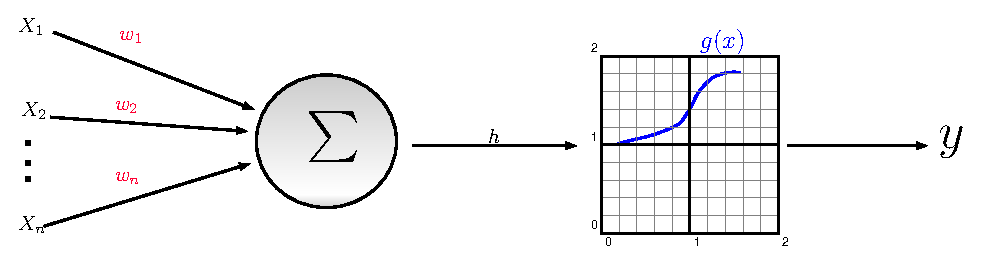
\includegraphics[scale=0.8]{Images/McCulloch.eps}
%	}
%	\caption{Modelo esquemático de um neurônio de McCulloch-Pitts. Onde $x_{1}, x_{2}, ..., x_{n}$ são os \textit{inputs}, $w_{1}, w_{2}, ..., w_{n}$ são os pesos, h é o treino, $g(x)$ é a função de ativação, e $y$ é o \textit{output}.}
%	\label{Esquematico de McCulloch}
%\end{figure*}

As redes alimentadas diretamente são aquelas redes cujos grafos orientados se distinguem pela presença de um ou mais camadas ocultas e cujos nós são chamados de neurônios ocultos. A função do neurônio é intervir entre a camada externa e a saída da rede de maneira útil. Adicionando-se camadas ocultas a rede torna-se capaz de realizar estatísticas de ordem elevada \citep{Haykin1999}.


\section{Resultados}
A região escolhida para a realização deste trabalho foi a $1$ localizada no centro do Rio de Janeiro. E o número de redes a serem testadas permaneceu $1$ para todos os testes. Foram realizados um total de $10$ diferentes testes. 

O janelamento utilizado no primeiro experimento foi de 12, com um codificação do mês real, uma topologia composta de 13 processadores, o algoritmo de treinamento "trainlm", com a função "tansig", e com uma função de saída linear, e sem a utilização do critério de parada antecipada. A Fig. \ref{topo1} apresenta à topologia da rede no primeiro experimento. 

\begin{figure}[H]
	\centering
	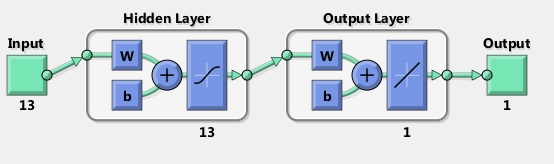
\includegraphics[scale=0.5]{Images/topologia1.jpg}
	\caption{Topologia da rede para o primeiro teste realizado.}
	\label{topo1}
\end{figure} 


O conjunto de treinamento, validação e teste para o primeiro experimento é apresentado na Fig. \ref{teste1}.

\begin{figure}[H]
	\centering
	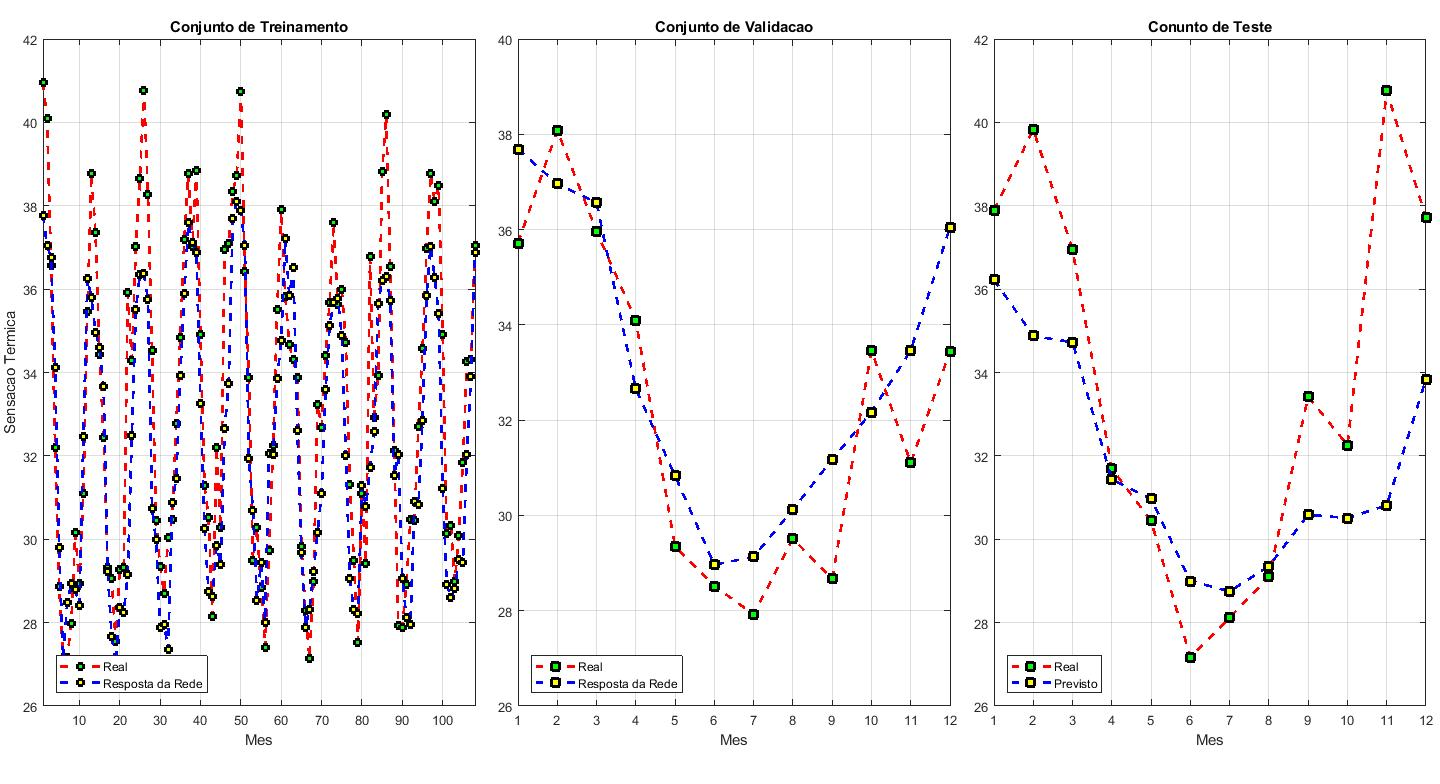
\includegraphics[scale=0.15]{Images/Teste1.jpg}
	\caption{Os gráficos apresentam da esquerda para a direita os conjuntos de treinamento, validação e teste da rede para o primeiro experimento. Em vermelho é registrado o dado real, enquanto em azul é apresentado o ajuste da rede. Aonde o eixo cartesiano horizontal representa os meses e o eixo vertical a sensação térmica.}
	\label{teste1}
\end{figure} 

O presente teste apresentou os seguintes valores de erros. MAPE de $4.2542$ para o conjunto de validação e $5.8434$ para o conjunto de treinamento. E valores de RMSE de $1.6624$ para o conjunto de validação e $2.7465$ para o conjunto de treinamento. 

O janelamento utilizado no segundo experimento foi de 6, com um codificação do mês real, uma topologia composta de 13 processadores, o algoritmo de treinamento "trainlm", com a função "tansig", e com uma função de saída linear, e sem a utilização do critério de parada antecipada. A Fig. \ref{topo2} apresenta à topologia da rede no segundo experimento. 

\begin{figure}[H]
	\centering
	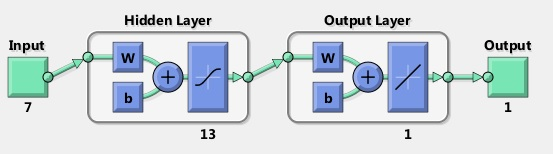
\includegraphics[scale=0.5]{Images/topologia2.jpg}
	\caption{Topologia da rede para o segundo teste realizado.}
	\label{topo2}
\end{figure} 


O conjunto de treinamento, validação e teste para o segundo experimento é apresentado na Fig. \ref{teste2}.

\begin{figure}[H]
	\centering
	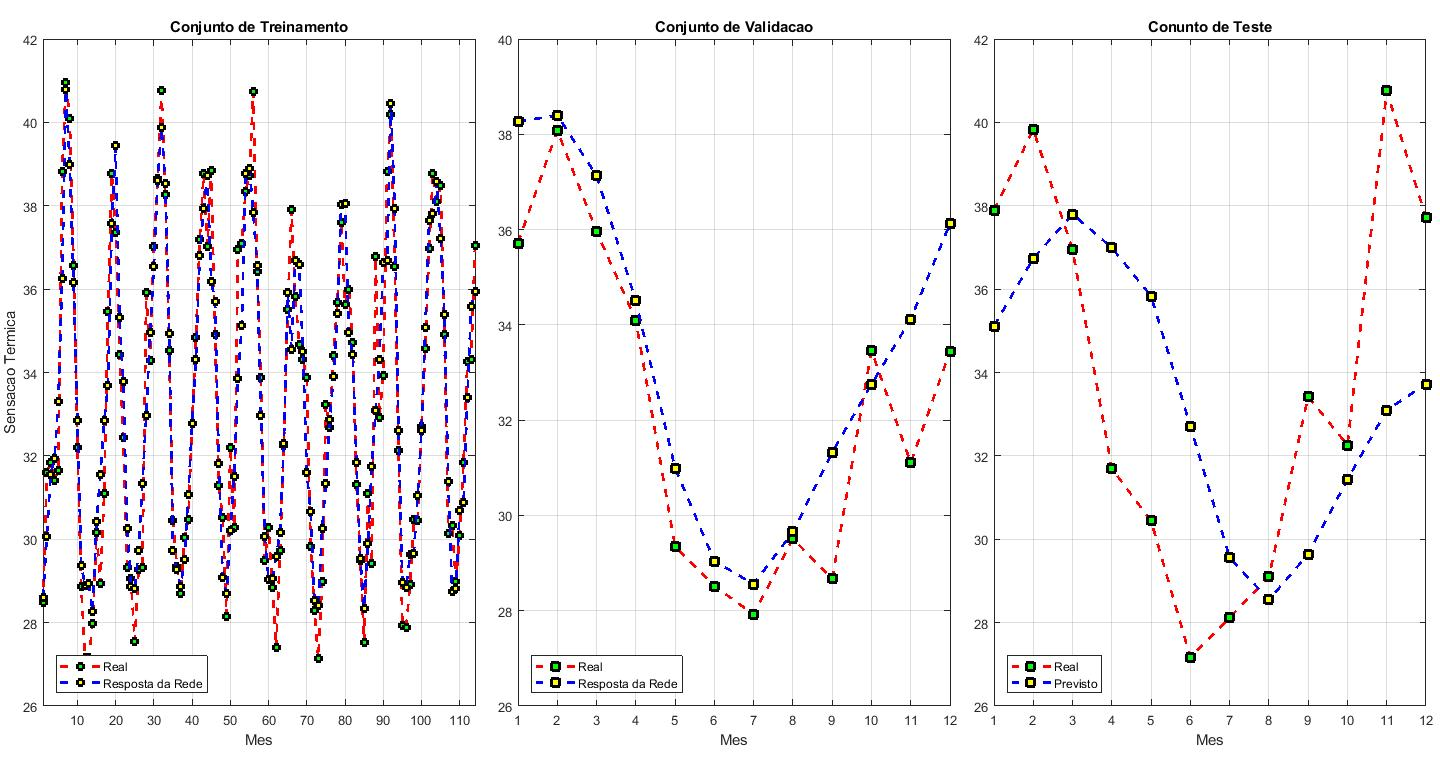
\includegraphics[scale=0.15]{Images/Teste2.jpg}
	\caption{Os gráficos apresentam da esquerda para a direita os conjuntos de treinamento, validação e teste da rede para o primeiro experimento. Em vermelho é registrado o dado real, enquanto em azul é apresentado o ajuste da rede. Aonde o eixo cartesiano horizontal representa os meses e o eixo vertical a sensação térmica.}
	\label{teste2}
\end{figure} 

O presente teste apresentou os seguintes valores de erros. MAPE de $4.7637$ para o conjunto de validação e $3.9691$ para o conjunto de treinamento. E valores de RMSE de $2.0730$ para o conjunto de validação e $2.1397$ para o conjunto de treinamento. 

O janelamento utilizado no terceiro experimento foi de 6, com um codificação do mês 4 bits, uma topologia composta de 13 processadores, o algoritmo de treinamento "trainlm", com a função "tansig", e com uma função de saída linear, e sem a utilização do critério de parada antecipada. A Fig. \ref{topo3} apresenta à topologia da rede no terceiro experimento. 

\begin{figure}[H]
	\centering
	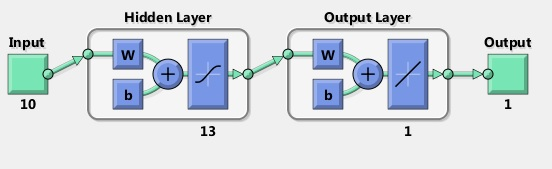
\includegraphics[scale=0.5]{Images/topologia3.jpg}
	\caption{Topologia da rede para o terceiro teste realizado.}
	\label{topo3}
\end{figure} 


O conjunto de treinamento, validação e teste para o terceiro experimento é apresentado na Fig. \ref{teste3}.

\begin{figure}[H]
	\centering
	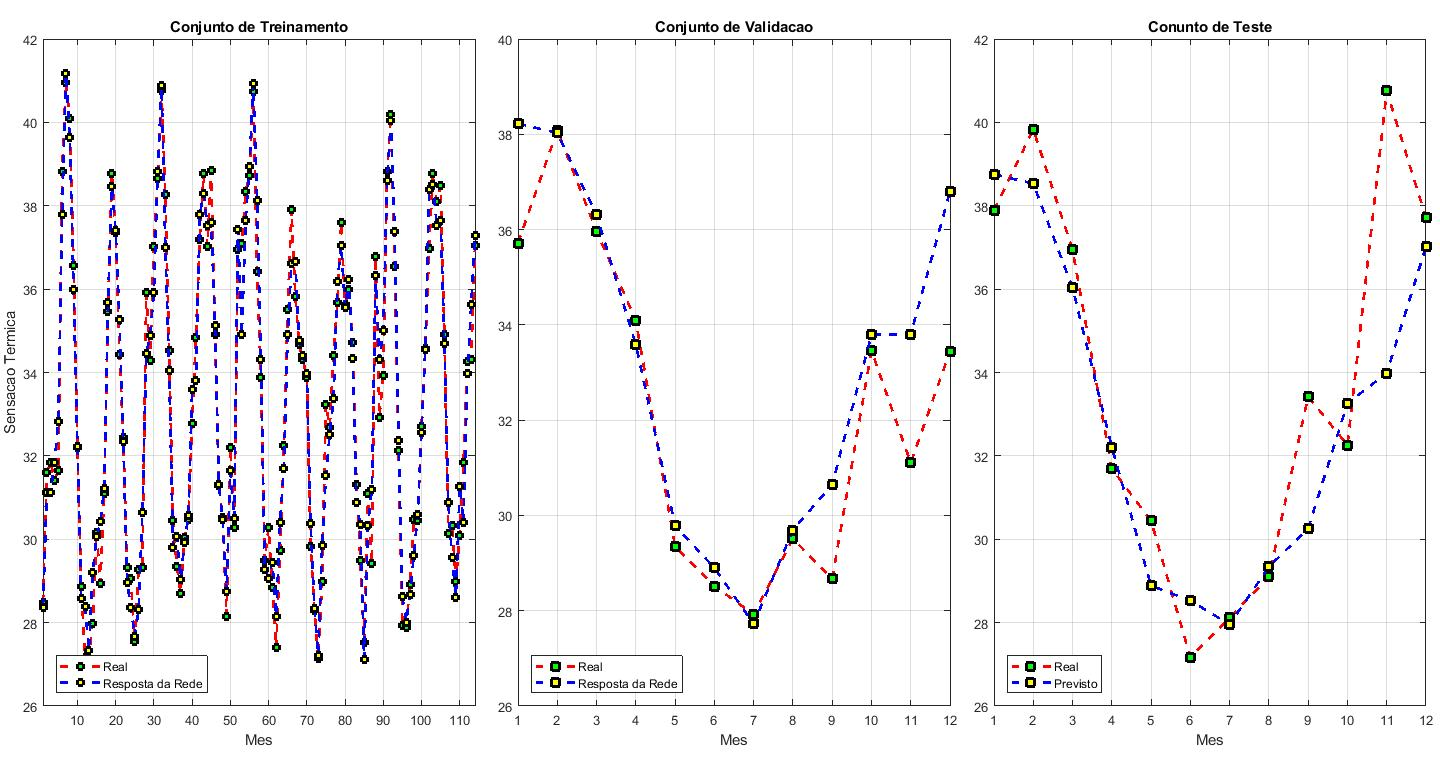
\includegraphics[scale=0.15]{Images/Teste3.jpg}
	\caption{Os gráficos apresentam da esquerda para a direita os conjuntos de treinamento, validação e teste da rede para o primeiro experimento. Em vermelho é registrado o dado real, enquanto em azul é apresentado o ajuste da rede. Aonde o eixo cartesiano horizontal representa os meses e o eixo vertical a sensação térmica.}
	\label{teste3}
\end{figure} 

O presente teste apresentou os seguintes valores de erros. MAPE de $3.3669$ para o conjunto de validação e $4.3468$ para o conjunto de treinamento. E valores de RMSE de $1.5717$ para o conjunto de validação e $2.3305$ para o conjunto de treinamento. 

O janelamento utilizado no quarto experimento foi de 6, com um codificação do mês 12 bits, uma topologia composta de 13 processadores, o algoritmo de treinamento "trainlm", com a função "tansig", e com uma função de saída linear, e sem a utilização do critério de parada antecipada. A Fig. \ref{topo4} apresenta à topologia da rede no quarto experimento. 

\begin{figure}[H]
	\centering
	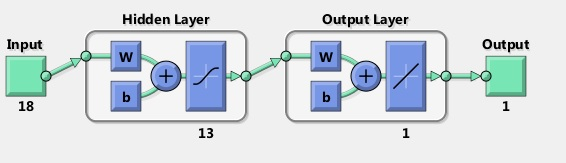
\includegraphics[scale=0.5]{Images/topologia4.jpg}
	\caption{Topologia da rede para o quarto teste realizado.}
	\label{topo4}
\end{figure} 


O conjunto de treinamento, validação e teste para o quarto experimento é apresentado na Fig. \ref{teste3}.

\begin{figure}[H]
	\centering
	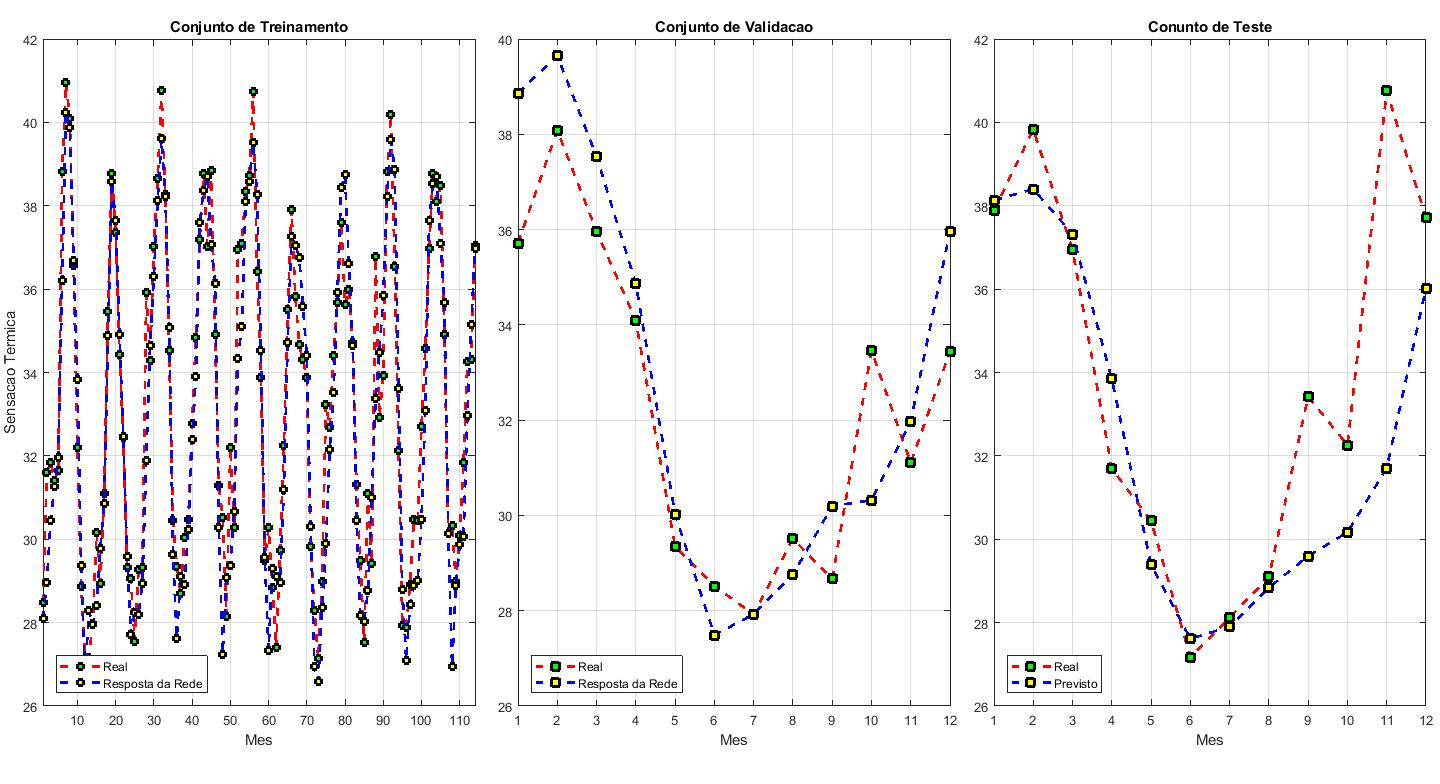
\includegraphics[scale=0.15]{Images/Teste4.jpg}
	\caption{Os gráficos apresentam da esquerda para a direita os conjuntos de treinamento, validação e teste da rede para o primeiro experimento. Em vermelho é registrado o dado real, enquanto em azul é apresentado o ajuste da rede. Aonde o eixo cartesiano horizontal representa os meses e o eixo vertical a sensação térmica.}
	\label{teste4}
\end{figure} 

O presente teste apresentou os seguintes valores de erros. MAPE de $4.4237$ para o conjunto de validação e $5.2831$ para o conjunto de treinamento. E valores de RMSE de $1.7508$ para o conjunto de validação e $3.0548$ para o conjunto de treinamento. 

O janelamento utilizado no quinto experimento foi de 6, com um codificação do mês 12 bits, uma topologia composta de $3$ processadores, o algoritmo de treinamento "trainlm", com a função "tansig", e com uma função de saída linear, e sem a utilização do critério de parada antecipada. A Fig. \ref{topo5} apresenta à topologia da rede no quinto experimento. 

\begin{figure}[H]
	\centering
	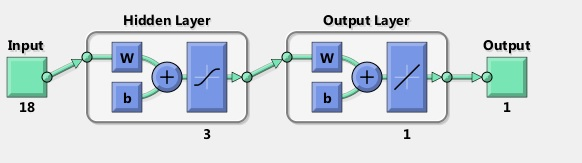
\includegraphics[scale=0.5]{Images/topologia5.jpg}
	\caption{Topologia da rede para o quinto teste realizado.}
	\label{topo5}
\end{figure} 


O conjunto de treinamento, validação e teste para o quinto experimento é apresentado na Fig. \ref{teste5}.

\begin{figure}[H]
	\centering
	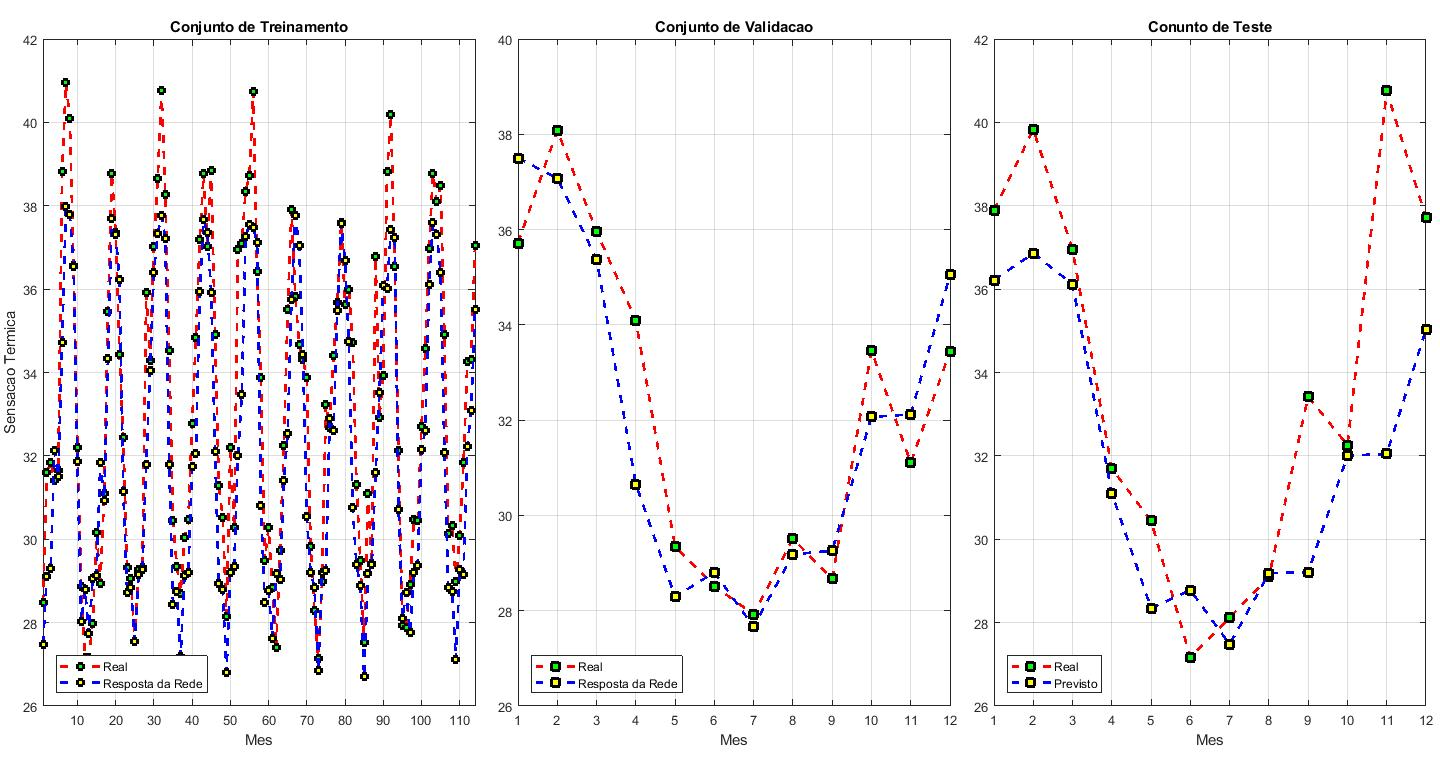
\includegraphics[scale=0.15]{Images/Teste5.jpg}
	\caption{Os gráficos apresentam da esquerda para a direita os conjuntos de treinamento, validação e teste da rede para o primeiro experimento. Em vermelho é registrado o dado real, enquanto em azul é apresentado o ajuste da rede. Aonde o eixo cartesiano horizontal representa os meses e o eixo vertical a sensação térmica.}
	\label{teste5}
\end{figure} 

O presente teste apresentou os seguintes valores de erros. MAPE de $3.3555$ para o conjunto de validação e $6.1024 $ para o conjunto de treinamento. E valores de RMSE de $1.4032$ para o conjunto de validação e $3.1737$ para o conjunto de treinamento. 

O janelamento utilizado no sexto experimento foi de 6, com um codificação do mês 12 bits, uma topologia composta de $23$ processadores, o algoritmo de treinamento "trainlm", com a função "tansig", e com uma função de saída linear, e sem a utilização do critério de parada antecipada. A Fig. \ref{topo6} apresenta à topologia da rede no sexto experimento. 

\begin{figure}[H]
	\centering
	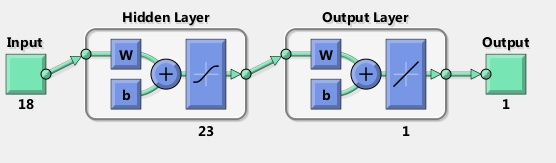
\includegraphics[scale=0.5]{Images/topologia6.jpg}
	\caption{Topologia da rede para o sexto teste realizado.}
	\label{topo6}
\end{figure} 


O conjunto de treinamento, validação e teste para o sexto experimento é apresentado na Fig. \ref{teste6}.

\begin{figure}[H]
	\centering
	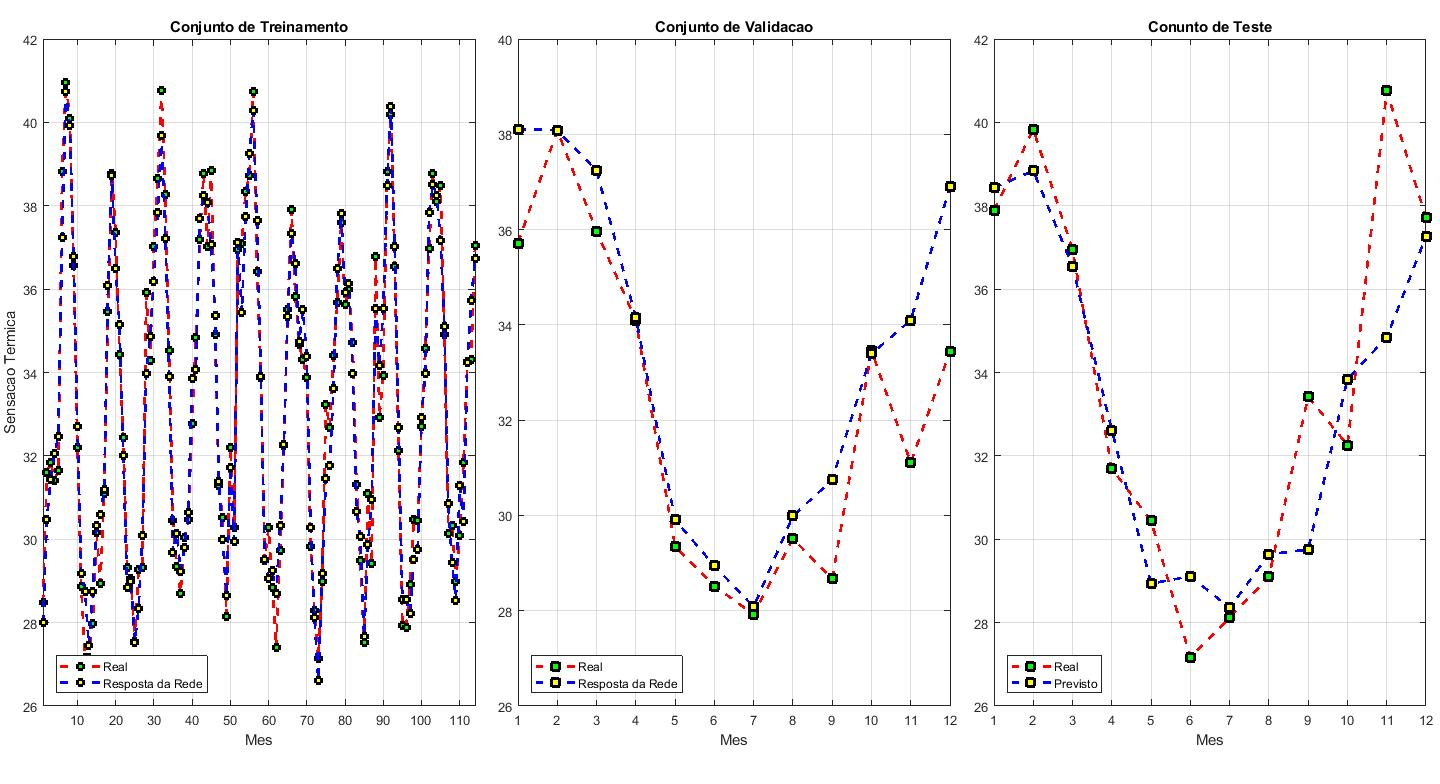
\includegraphics[scale=0.15]{Images/Teste6.jpg}
	\caption{Os gráficos apresentam da esquerda para a direita os conjuntos de treinamento, validação e teste da rede para o primeiro experimento. Em vermelho é registrado o dado real, enquanto em azul é apresentado o ajuste da rede. Aonde o eixo cartesiano horizontal representa os meses e o eixo vertical a sensação térmica.}
	\label{teste6}
\end{figure} 

O presente teste apresentou os seguintes valores de erros. MAPE de $3.6180$ para o conjunto de validação e $4.5186$ para o conjunto de treinamento. E valores de RMSE de $1.6659$ para o conjunto de validação e $2.2323$ para o conjunto de treinamento. 

O janelamento utilizado no sétimo experimento foi de 6, com um codificação do mês 12 bits, uma topologia composta de $23$ processadores, o algoritmo de treinamento "trainlm", com a função "logsig", e com uma função de saída linear, e sem a utilização do critério de parada antecipada. A Fig. \ref{topo7} apresenta à topologia da rede no sétimo experimento. 

\begin{figure}[H]
	\centering
	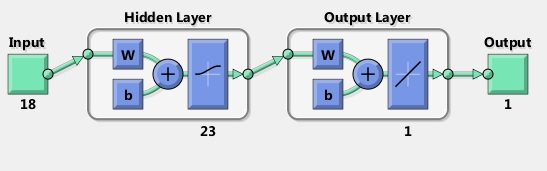
\includegraphics[scale=0.5]{Images/topologia7.jpg}
	\caption{Topologia da rede para o sétimo teste realizado.}
	\label{topo7}
\end{figure} 


O conjunto de treinamento, validação e teste para o sétimo experimento é apresentado na Fig. \ref{teste7}.

\begin{figure}[H]
	\centering
	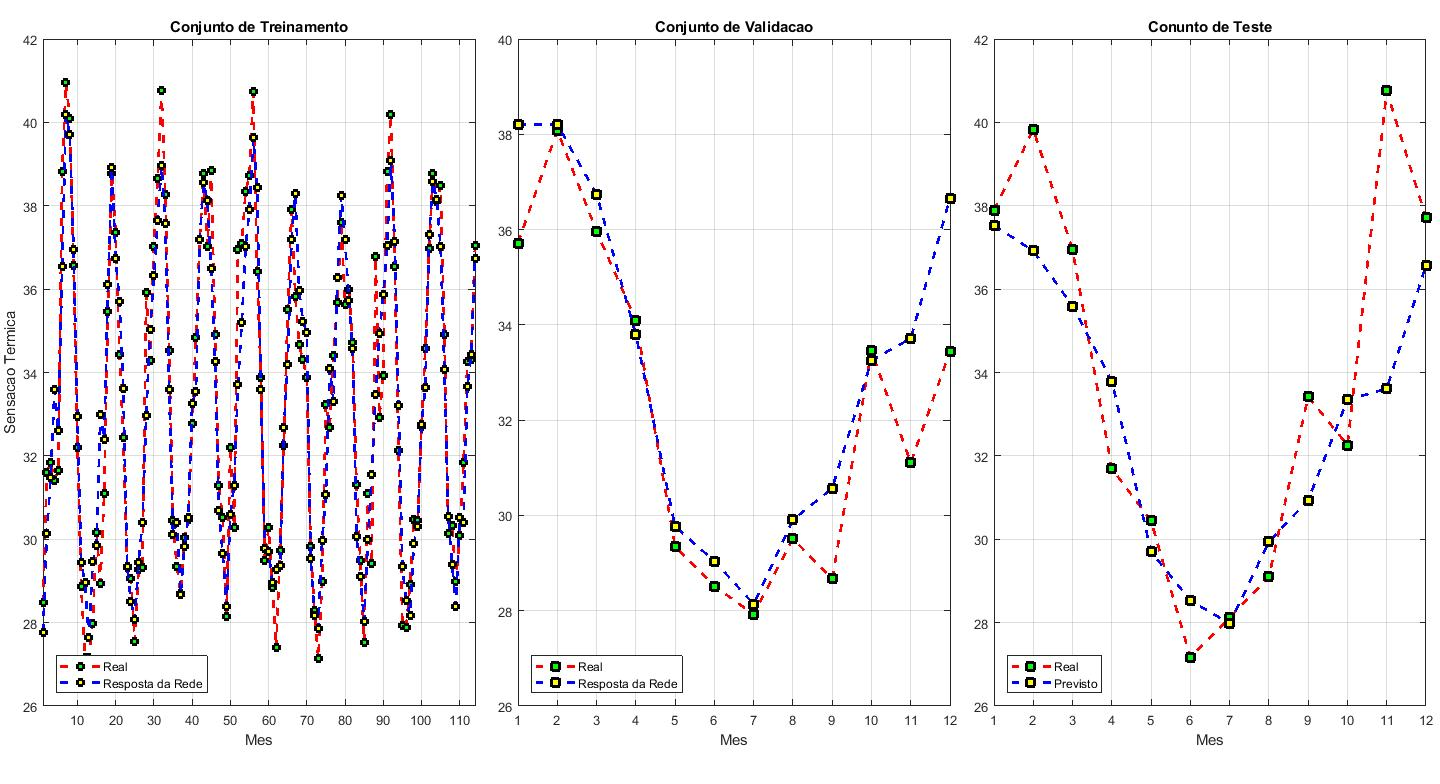
\includegraphics[scale=0.15]{Images/Teste7.jpg}
	\caption{Os gráficos apresentam da esquerda para a direita os conjuntos de treinamento, validação e teste da rede para o primeiro experimento. Em vermelho é registrado o dado real, enquanto em azul é apresentado o ajuste da rede. Aonde o eixo cartesiano horizontal representa os meses e o eixo vertical a sensação térmica.}
	\label{teste7}
\end{figure} 

O presente teste apresentou os seguintes valores de erros. MAPE de $3.4132$ para o conjunto de validação e $5.0634$ para o conjunto de treinamento. E valores de RMSE de $1.5364$ para o conjunto de validação e $2.5437$ para o conjunto de treinamento.

O janelamento utilizado no oitavo experimento foi de 6, com um codificação do mês 12 bits, uma topologia composta de $23$ processadores, o algoritmo de treinamento "trainlm", com a função "logsig", e com uma função de saída "logsig", e sem a utilização do critério de parada antecipada. A Fig. \ref{topo8} apresenta à topologia da rede no oitavo experimento. 

\begin{figure}[H]
	\centering
	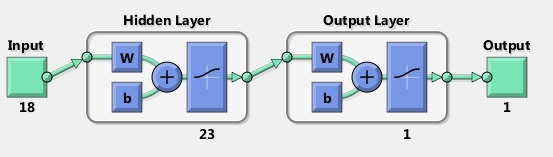
\includegraphics[scale=0.5]{Images/topologia8.jpg}
	\caption{Topologia da rede para o oitavo teste realizado.}
	\label{topo8}
\end{figure} 


O conjunto de treinamento, validação e teste para o oitavo experimento é apresentado na Fig. \ref{teste8}.

\begin{figure}[H]
	\centering
	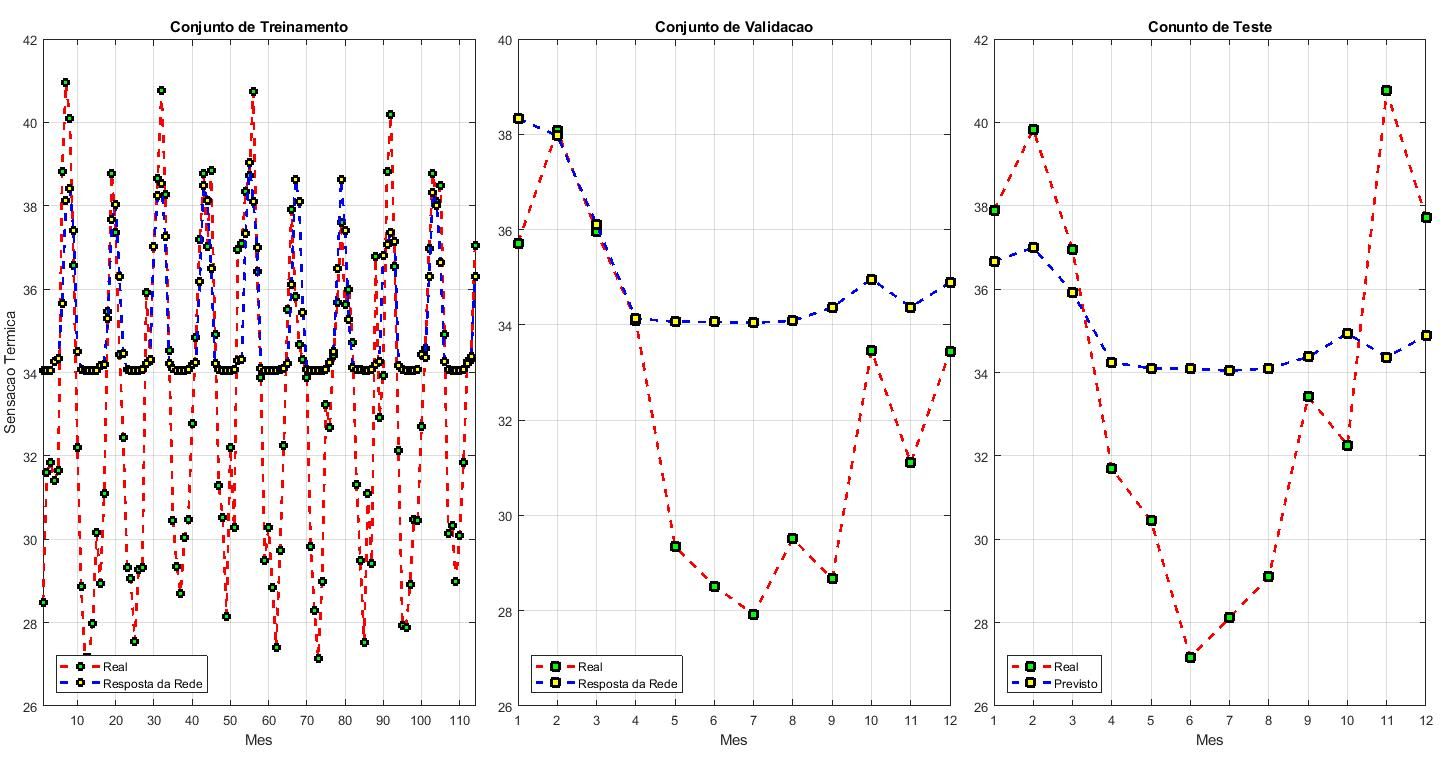
\includegraphics[scale=0.15]{Images/Teste8.jpg}
	\caption{Os gráficos apresentam da esquerda para a direita os conjuntos de treinamento, validação e teste da rede para o primeiro experimento. Em vermelho é registrado o dado real, enquanto em azul é apresentado o ajuste da rede. Aonde o eixo cartesiano horizontal representa os meses e o eixo vertical a sensação térmica.}
	\label{teste8}
\end{figure} 

O presente teste apresentou os seguintes valores de erros. MAPE de $10.0192$ para o conjunto de validação e $10.9309$ para o conjunto de treinamento. E valores de RMSE de $3.7165$ para o conjunto de validação e $4.0335$ para o conjunto de treinamento.

O janelamento utilizado no nono experimento foi de 6, com um codificação do mês 12 bits, uma topologia composta de $23$ processadores, o algoritmo de treinamento "trainlm", com a função "logsig", e com uma função de saída "logsig", e com a utilização do critério de parada antecipada. A Fig. \ref{topo9} apresenta à topologia da rede no nono experimento. 

\begin{figure}[H]
	\centering
	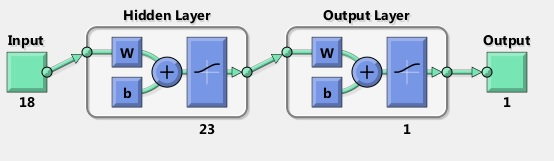
\includegraphics[scale=0.5]{Images/topologia9.jpg}
	\caption{Topologia da rede para o nono teste realizado.}
	\label{topo9}
\end{figure} 


O conjunto de treinamento, validação e teste para o nono experimento é apresentado na Fig. \ref{teste9}.

\begin{figure}[H]
	\centering
	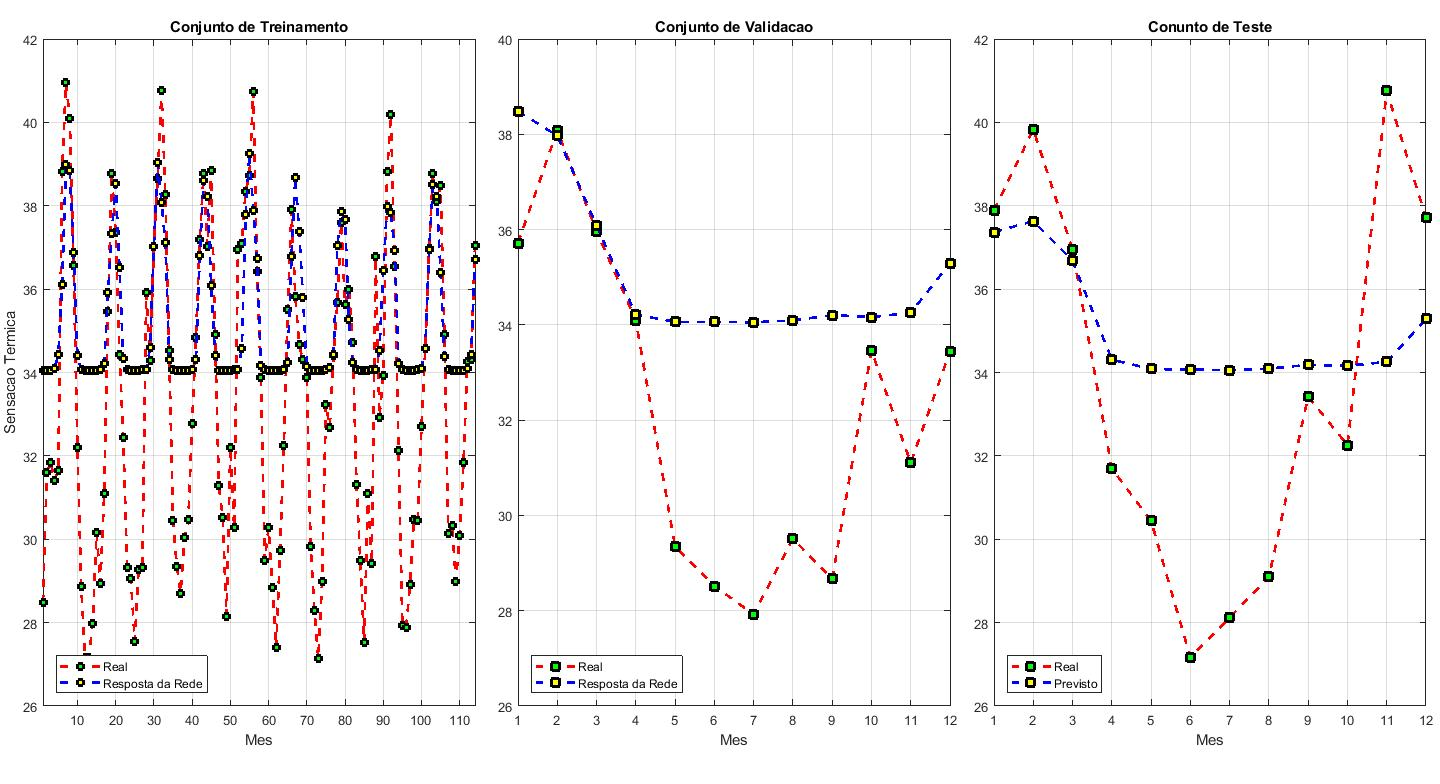
\includegraphics[scale=0.15]{Images/Teste9.jpg}
	\caption{Os gráficos apresentam da esquerda para a direita os conjuntos de treinamento, validação e teste da rede para o primeiro experimento. Em vermelho é registrado o dado real, enquanto em azul é apresentado o ajuste da rede. Aonde o eixo cartesiano horizontal representa os meses e o eixo vertical a sensação térmica.}
	\label{teste9}
\end{figure} 

O presente teste apresentou os seguintes valores de erros. MAPE de $9.8988$ para o conjunto de validação e $10.1712$ para o conjunto de treinamento. E valores de RMSE de $3.6942$ para o conjunto de validação e $3.9312$ para o conjunto de treinamento.

No final deste relatório é apresentado um quadro geral de todos os testes realizados.

\begin{figure*}[ht!]
	\centering
	\subfloat[Experimento 1]{
		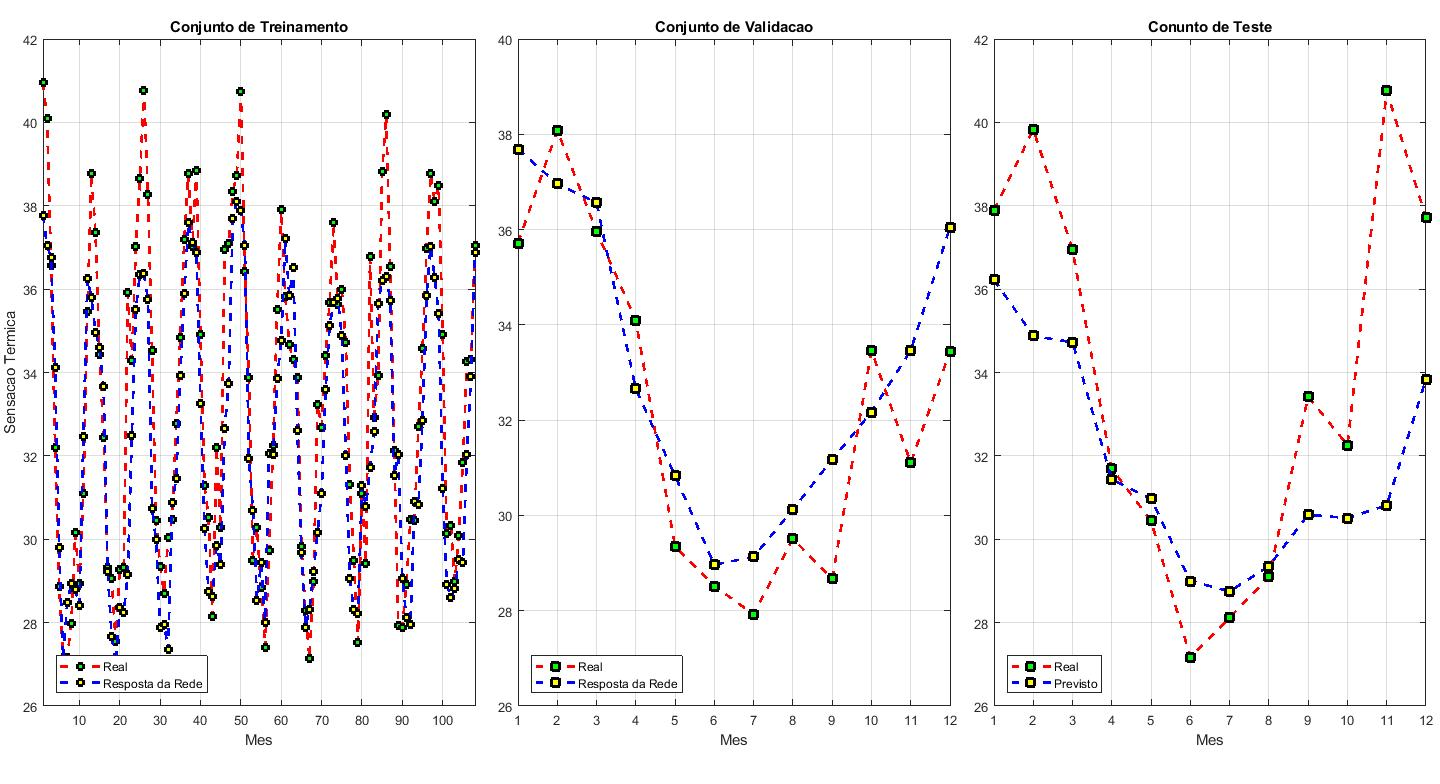
\includegraphics[height=8cm]{Images/Teste1.jpg}
	}
	\quad %espaco separador
	\subfloat[Experimento 2]{
		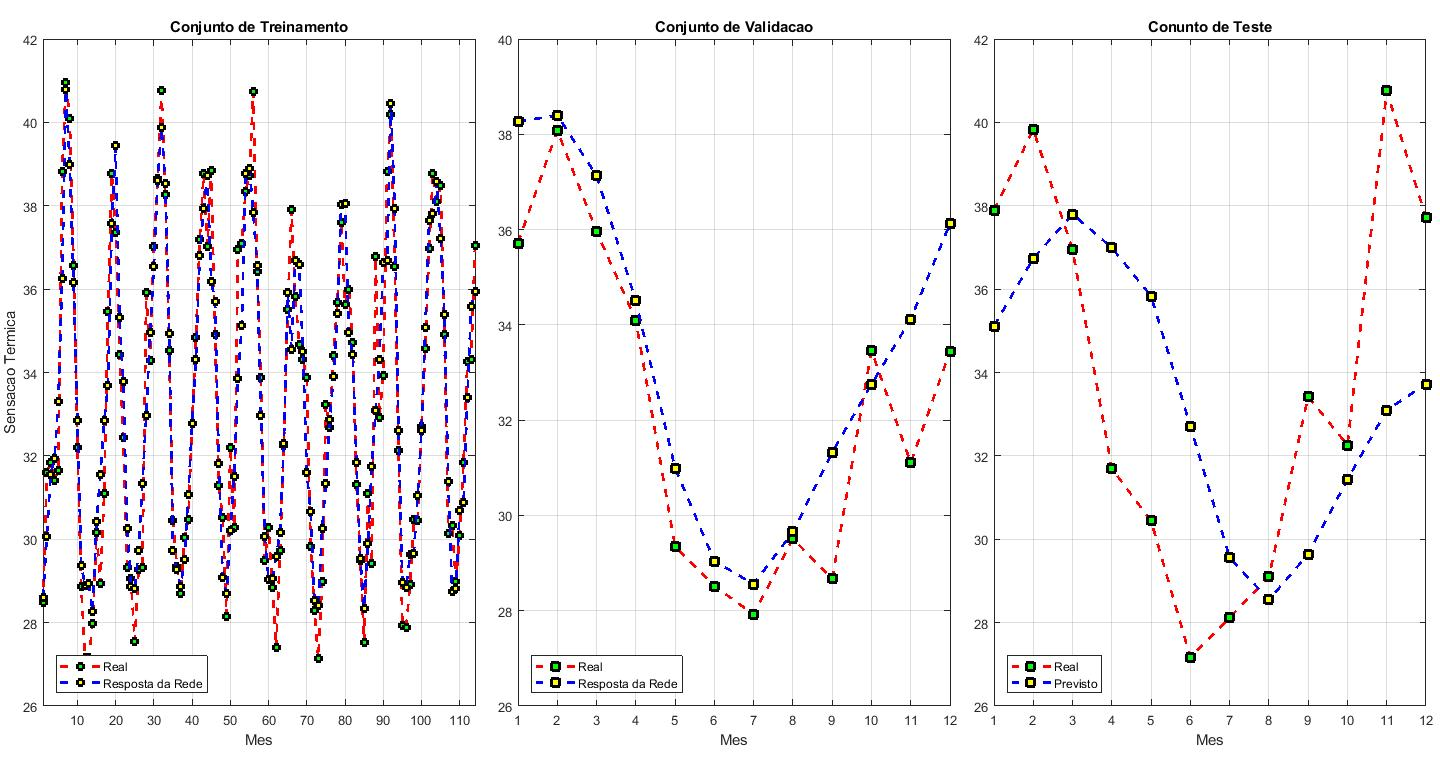
\includegraphics[height=8cm]{Images/Teste2.jpg}
	}
	\quad %espaco separador
	\subfloat[Experimento 3]{
		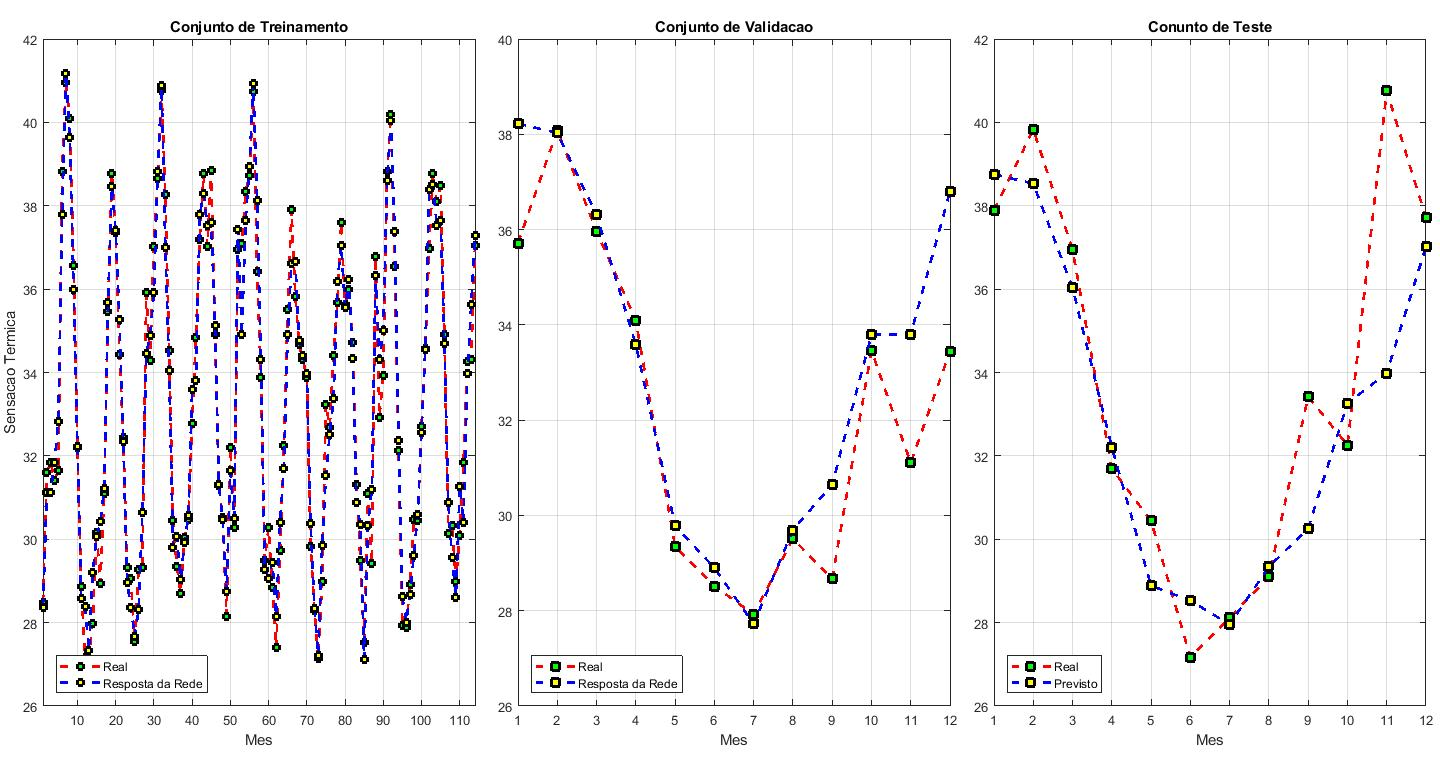
\includegraphics[height=8cm]{Images/Teste3.jpg}
	}
    \caption{Quadro geral de testes. Da primeira para a última tríades de gráficos estão apresentadas na ordem crescente de experimentos que vão do $1-3$. }
\end{figure*}


\begin{figure*}[ht!]
	\centering
    \subfloat[Experimento 4]{
       	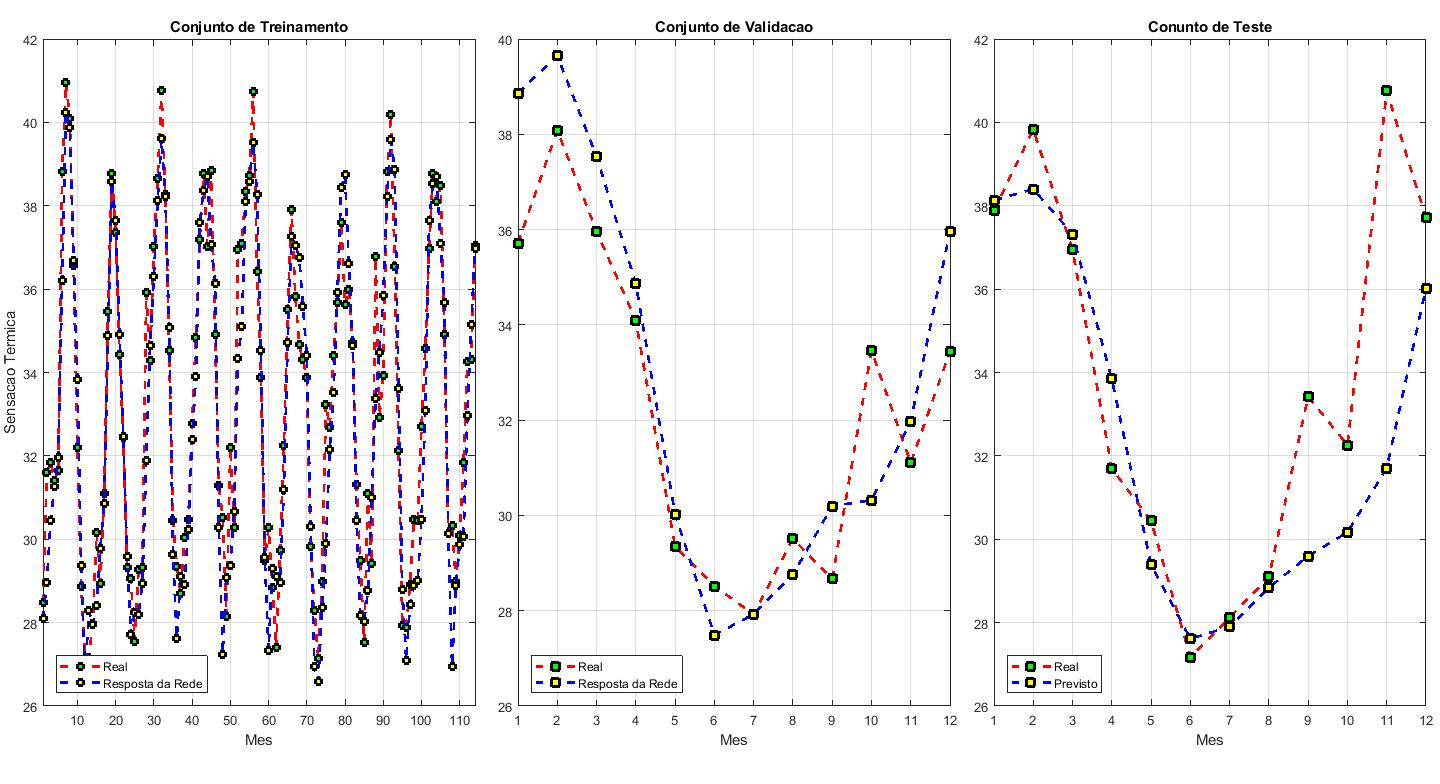
\includegraphics[height=8cm]{Images/Teste4.jpg}
    }
    \quad %espaco separador
    \subfloat[Experimento 5]{
	    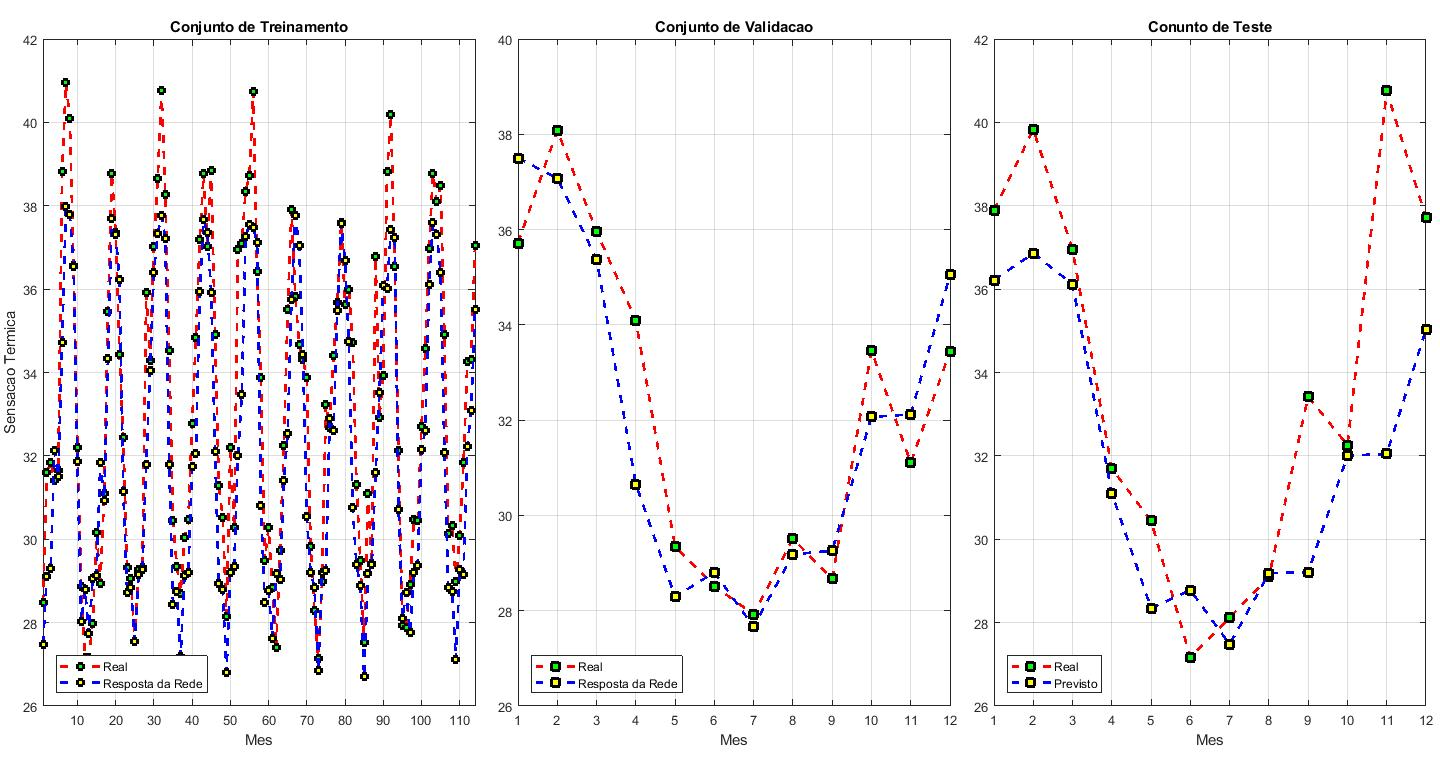
\includegraphics[height=8cm]{Images/Teste5.jpg}
    }
    \quad %espaco separador
    \subfloat[Experimento 6]{
    	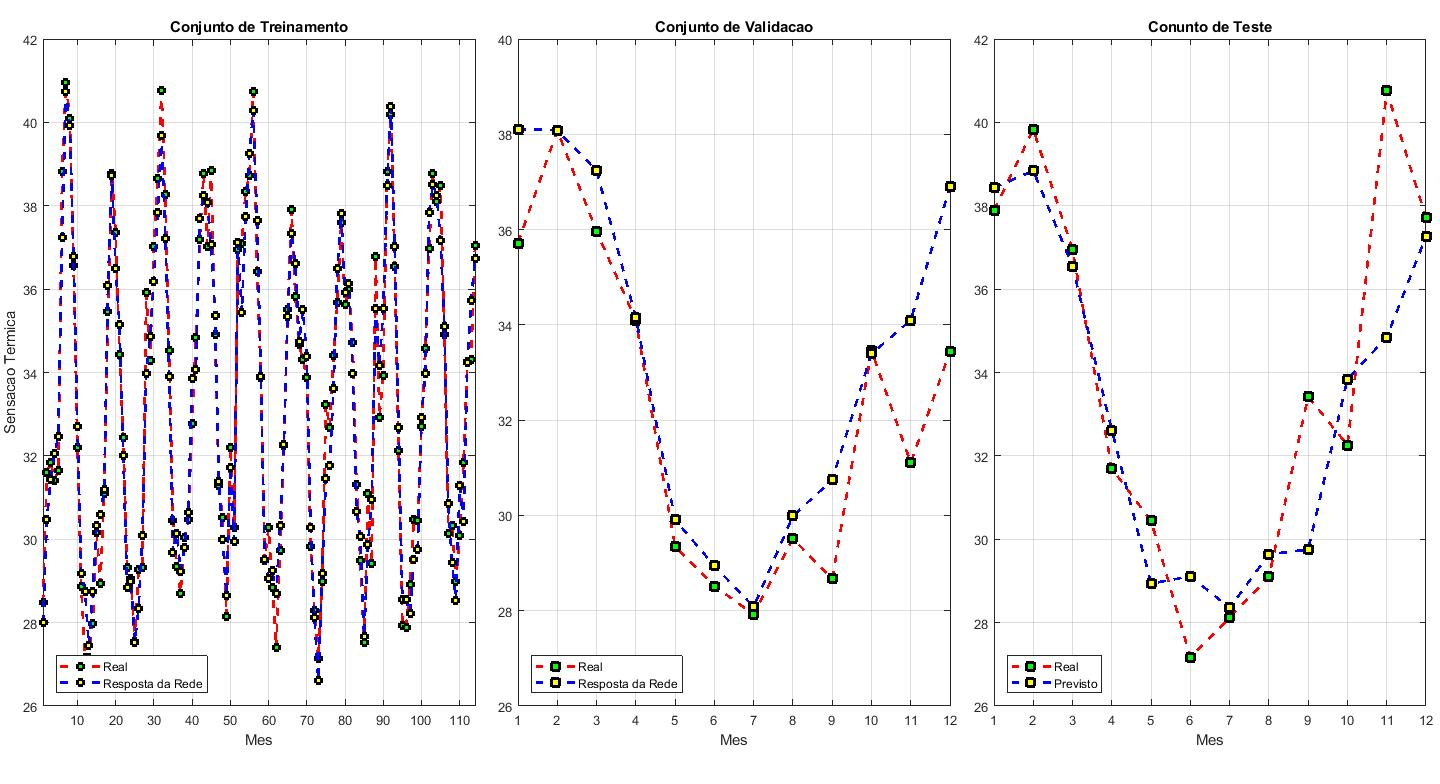
\includegraphics[height=8cm]{Images/Teste6.jpg}
    }
    \caption{Quadro geral de testes. Da primeira para a última tríades de gráficos estão apresentadas na ordem crescente de experimentos que vão do $4-6$. }
\end{figure*}


\begin{figure*}[ht!]
	\centering
    \subfloat[Experimento 7]{
    	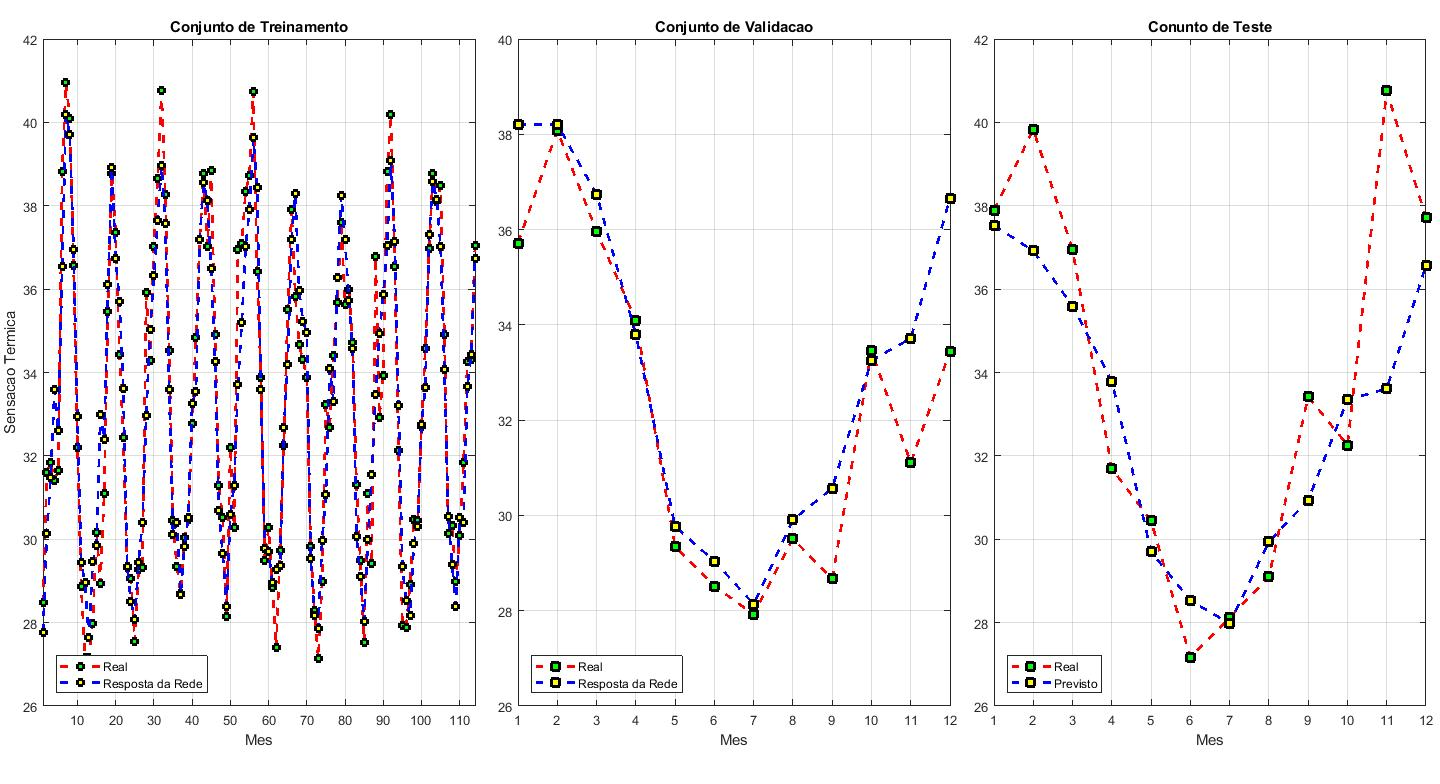
\includegraphics[height=8cm]{Images/Teste7.jpg}
    }
    \quad %espaco separador
    \subfloat[Experimento 8]{
    	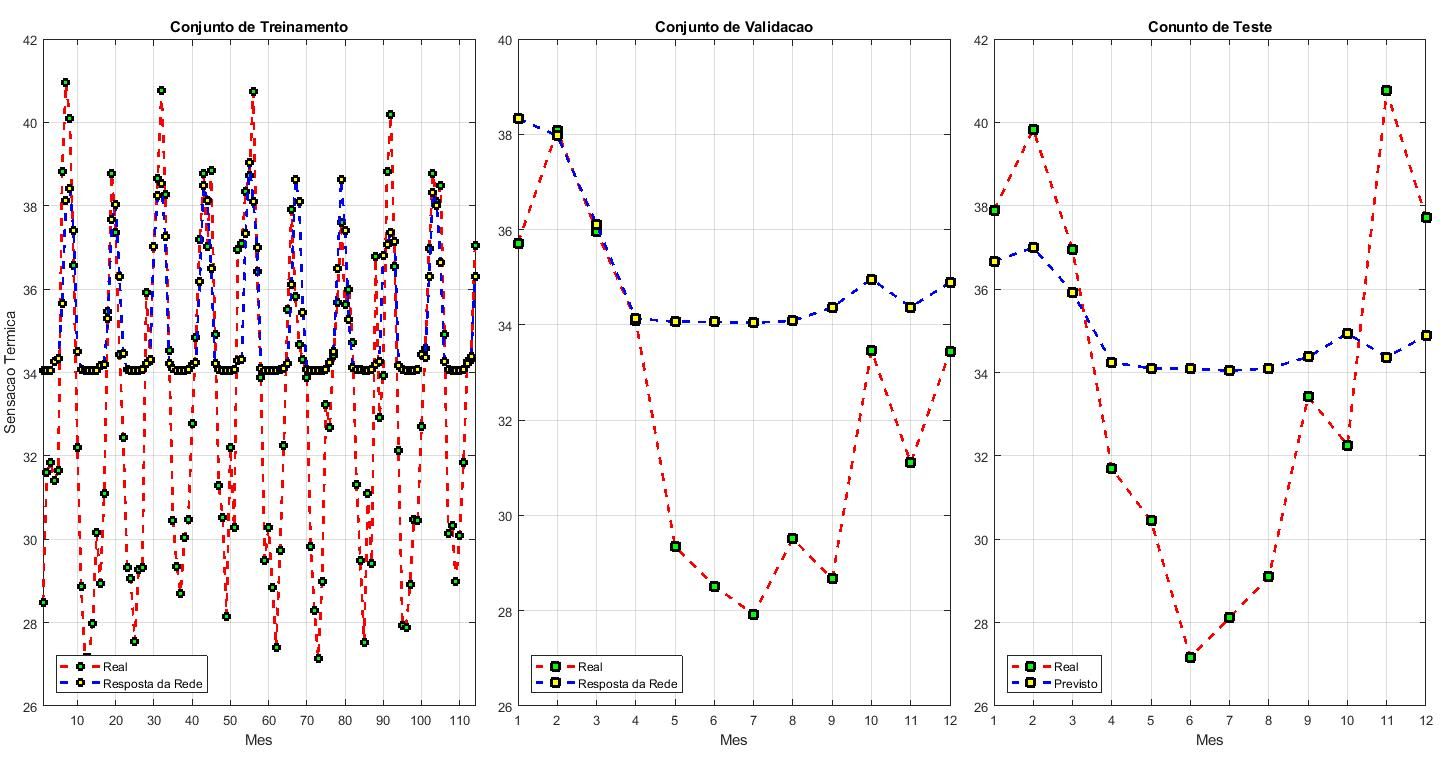
\includegraphics[height=8cm]{Images/Teste8.jpg}
    }
    \quad %espaco separador
    \subfloat[Experimento 9]{
    	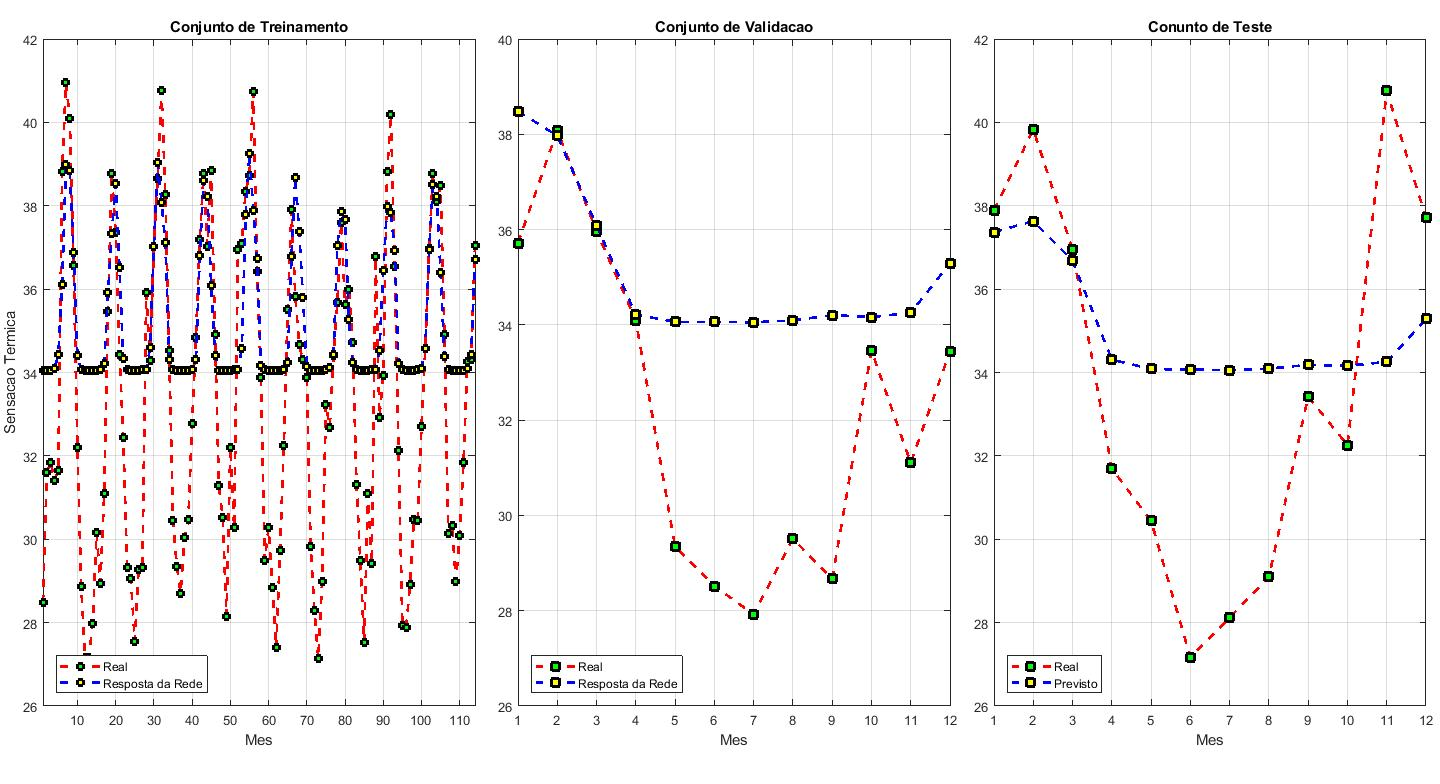
\includegraphics[height=8cm]{Images/Teste9.jpg}
    }
    \caption{Quadro geral de testes. Da primeira para a última tríades de gráficos estão apresentadas na ordem crescente de experimentos que vão do $7-9$. }
\end{figure*}


\section{Conclusões}


Os experimentos realizados apresentam uma sequência lógica de alterações de parâmetros da rede. Isto é, somente um parâmetro é alterado por vez, enquanto os demais permanecem inalterados. 

Dentre esta sequência de experimentos o que apresentou o melhor resultado foi experimento de número três, cujo janelamento utilizado foi o de 6, com um codificação do mês 4 bits, uma topologia composta de $13$ processadores, o algoritmo de treinamento "trainlm", com a função "tansig", e com uma função de saída linear, e sem a utilização do critério de parada antecipada.  Este apresentou erros de MAPE de $3.3669$ para o conjunto de validação e $4.3468$ para o conjunto de treinamento. E valores de RMSE de $1.5717$ para o conjunto de validação e $2.3305$ para o conjunto de treinamento.

Em contrapartida, o experimento que apresentou o pior desempenho foi o oitavo cujo janelamento utilizado foi de 6, com um codificação do mês 12 bits, uma topologia composta de $23$ processadores, o algoritmo de treinamento "trainlm", com a função "logsig", e com uma função de saída "logsig", e sem a utilização do critério de parada antecipada. Apresentando erros de MAPE de $10.0192$ para o conjunto de validação e $10.9309$ para o conjunto de treinamento. E valores de RMSE de $3.7165$ para o conjunto de validação e $4.0335$ para o conjunto de treinamento.

Essa discrepância registrada se deveu principalmente ao fato de que o experimento $3$ possui uma janela de previsão menor do que o experimento $8$. Outro fator importante para o aumento dos erros foi a utilização do critério de parada antecipada no experimento $8$. Como neste caso o número de processadores foi aumentado para $23$ seria necessário aumentar o número de ciclos de treinamento ou diminuir o critério de parada. 

Outra questão iportante foi a mudança da função de saída de linear para "logsig".A função linear possui um comportamento sem grandes variações entre os pontos que a descrevem. Enquanto que a função "logsig" já apresenta um comportamento mais variável. Soma-se a isso ao fato de a natureza do dado escolhido (centro do Rio de Janeiro) apresentar pouca variação no comportamento de temperatura ao longo dos meses se comparado com outras regiões da cidade. 

% Now we need a bibliography:


\bibliographystyle{apalike}
\bibliography{references}


% Your document ends here!
\end{document}